\newpage
\section{Extraktion der Zitate}\label{citation-extraction}

Die vorliegende Auswertung bezüglich der Anzahl Zitate von Männern und Frauen pro Nachrichtenportal
fokussiert sich auf das Erkennen und Extrahieren der sogenannten \textsl{Syntaktischen Zitate}.
Der Grund dafür ist, dass diese von der Form her die klarste Struktur aufweisen und auch die Basis
für das Erkennen der anderen Arten von Zitaten darstellen.

Weitere Arten von Zitaten, die in dieser Arbeit aufgrund des zeitlichen Rahmens nicht berücksichtigt
werden konnten sind
\begin{enumerate}
    \item \textsl{Schwimmende Zitate},
    \item \textsl{Heuristische Zitate} und
    \item \textsl{Syntaktische Zitate}, die ein zu unspezifisches oder gar kein Verb enthalten.
Das können Zitate sein, die mit \enquote{gemäss} oder \enquote{so} usw. eingeleitet werden.
\end{enumerate}

Nachfolgend ist deshalb ausschliesslich die Extraktion der \textsl{Syntaktischen Zitate} mit spezifischen
Verben beschrieben. Auf die weiteren Arten und deren mögliche Erkennung wird im Kapitel
\ref{further-research} eingegangen.

Die \textsl{Syntaktischen Zitate} zeichnen sich in der Textanalyse mit \gl{spacy-parser} 
dadurch aus, dass sie im resultierenden Parse Tree in einer fast eindeutigen Struktur auftauchen
und deshalb mit einem klar definierten Regelwerk extrahiert werden können. Beispiele dazu finden sich
in den nachfolgenden Unterkapiteln.

\subsection{Parse Trees}

Die Analyse eines Texts (Strings) mit dem \gl{spacy-parser} resultiert in einer Baumstruktur,
welche die Abhängigkeit der Wörter untereinander enthält. Die Aufgabe des Programms besteht also
darin, Subtrees einer gewissen Struktur zu erkennen. Die Abbildung \ref{tree-general} ist eine
Abstraktion eines solchen Subtrees.

In den eckigen Klammern ist die Art des Worts beschrieben. Diese wird gefolgt von einem Bodenstrich (\_)
und der \gl{spacy} -Abkürzung für die Kategorie des Worts.



\begin{figure}[H]
	\begin{center}
        \centering
		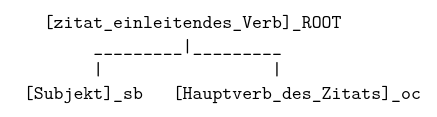
\includegraphics[width=0.6\linewidth]{./images/structure_citation.png}
	\end{center}
\caption{Subtree Repräsentation eines Syntaktischen Zitats}
\label{tree-general}
\end{figure}

Die möglichen Kategorien sind in der Tabelle \ref{legend-spacy-parsers} beschrieben. Diese Kategorien
widerspiegeln nicht konsequent Wortarten oder Begriffe aus der Satzlehre, wie sie im Deutschunterricht
gelehrt werden. Deshalb ist auch mit der Erklärung oft nicht klar, wofür sie stehen. Deren Auftreten
ist jedoch konsistent genug, sodass sie zur Erkennung der gewünschten Satzstrukturen genutzt werden
können.

\begin{table}[H]
    \centering
    \begin{tabular}{|l|r|}
        \hline
        \textbf{Spacy Parser Label} & \textbf{Spacy Erklärung} \\
        \hline
        \hline
        ROOT & root \\
        \hline
        da & dative \\
        \hline
        mnr & postnominal modifier \\
        \hline
        mo & modifier \\
        \hline
        nk & noun kernel element \\
        \hline
        oc & clausal object \\
        \hline
        punct & punctuation \\
        \hline
        sb & subject \\
        \hline
    \end{tabular}
    \caption{Legende zu den wichtigsten Spacy Parser Labels}
    \label{legend-spacy-parsers}
\end{table}

Die nachfolgenden Abbildungen \ref{tree-direct} und \ref{tree-indirect} sind konkrete Beispiele solcher
Trees. Der \gl{spacy-parser}  überrascht mit seiner Fähigkeit, Zitate in der direkten und
indirekten Rede gleich strukturieren zu können.

Die Abbildung \ref{tree-direct} repräsentiert den Satz
\enquote{Macron sagte zu Xi, »Die Aggression hat der Stabilität einen Schlag versetzt«.}
mit einem Zitat in der direkten Rede.

\begin{figure}[H]
	\begin{center}
        \centering
		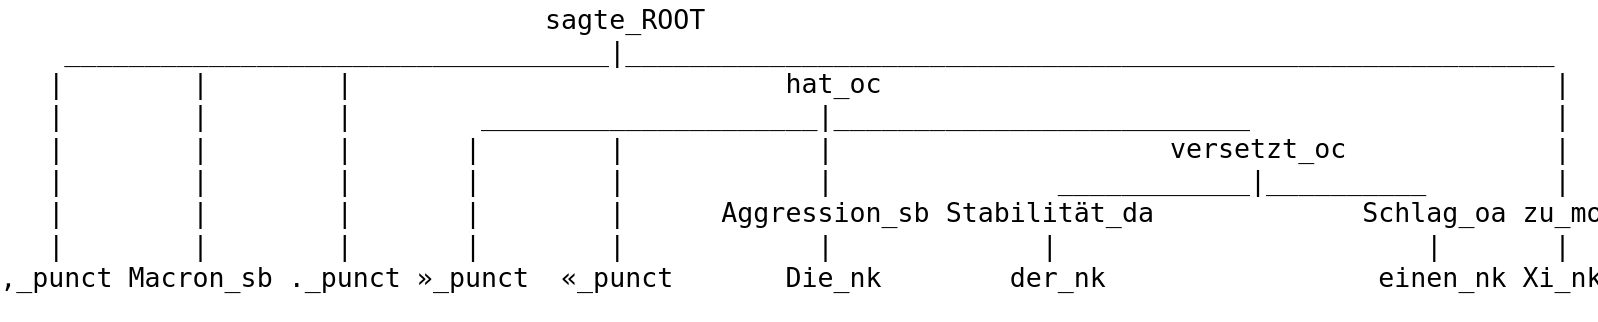
\includegraphics[width=\linewidth]{./images/macron-sagte-zu-xi-direkt.png}
	\end{center}
\caption{Parse Tree eines Satzes mit einem Syntaktischem Zitat in der direkten Rede}
\label{tree-direct}
\end{figure}

Die Abbildung \ref{tree-indirect} repräsentiert den Satz
\enquote{Macron sagte zu Xi dass die Aggression der Stabilität einen Schlag versetzt habe.}
mit einem Zitat in der indirekten Rede.

\begin{figure}[H]
	\begin{center}
        \centering
		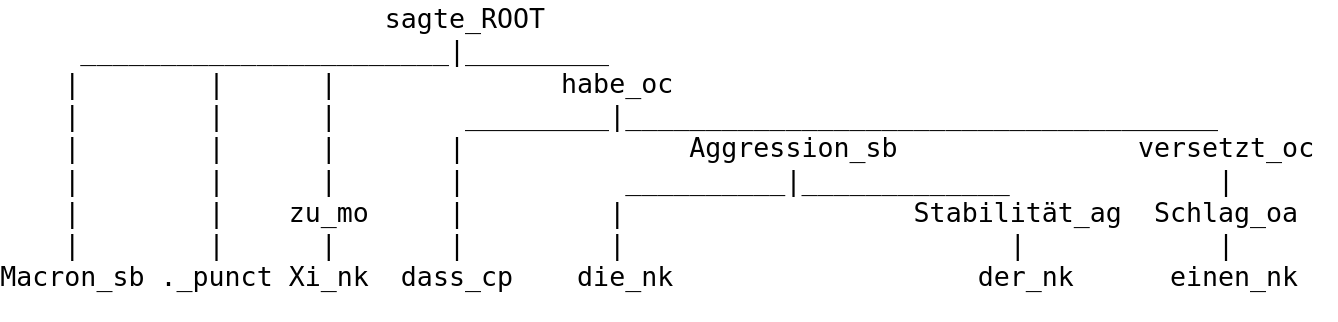
\includegraphics[width=\linewidth]{./images/macron-sagte-zu-xi-indirekt.png}
	\end{center}
\caption{Parse Tree eines Satzes mit einem Syntaktischem Zitat in der indirekten Rede.}
\label{tree-indirect}
\end{figure}

\subsection{Ablauf des Algorithmus}

Der nachfolgende Abschnitt soll konzeptuell und mit einigen Code-Beispielen erklären, wie der
Algorithmus vorgeht, um die Zitate in der oben beschriebenen Struktur zu Erkennen und zu extrahieren.

Hinweis: Im nachfolgenden Text werden die Terme \enquote{Node}, \enquote{Knoten} und \enquote{Token} als Synonyme verwendet.
Der Grund dafür ist, dass \enquote{Token} die Namensgebung von \gl{spacy}  ist und \enquote{Node} und \enquote{Knoten}
die passenden Begriffe dazu aus der Graphentheorie sind.

Der nachfolgende Code in Abbildung \ref{get-quotation-node} zeigt die Funktion, die das Programm verwendet,
um den \enquote{Hauptverb des Zitats} (vgl. Abbildung \ref{tree-general})
aus dem Parse Tree zu extrahieren. Gemeint ist damit derjenige Knoten, der als Kinder alle Wörter 
des Zitats enthält. Grundsätzlich muss die Funktion dabei unterscheiden, ob der vorliegende Satz 
in einer Zeitform mit Hilfsverb vorliegt (Perfekt, Plusquamperfekt oder Futur) oder in einer 
Zeitform ohne (Präsens oder Präteritum).

Die Funktion bedient sich einer weiteren Funktion \enquote{\_\_get\_nearest\_token\_by\_condition}
(vgl. Abbildung \ref{get-token-by-condition}), um in einer Breitensuche nach dem entsprechenden Node zu suchen.

\begin{figure}[H]
    \begin{lstlisting}[language=Python]
def __get_quote_node(root: Token) -> Token:
    result = []

    # Perfekt, Plusquamperfekt, Futur
    if root.lemma_ in __get_hilfsverben():
        condition = (
            lambda n: n.head.lemma_ in __get_quotation_verbs() and n.dep_ == "oc"
        )
        result = __get_flattened_list(
            [__get_nearest_tokens_by_condition(c, condition) for c in root.children]
        )

    # Präsens, Präteritum
    if root.lemma_ in __get_quotation_verbs():
        result = [x for x in root.children if x.dep_ == "oc"]

    if len(result) < 1:
        raise _NotFoundError()

    return result[0]
    \end{lstlisting}
    \caption{Function \_\_get\_quote\_node}
    \label{get-quotation-node}
\end{figure}

Die Funktion \enquote{\_\_get\_nearest\_token\_by\_condition} in der Abbildung \ref{get-token-by-condition} wird vom Algorithmus verwendet,
um die Knoten des Subjekts, des Zitat-einleitenden Verbes und des Zitats zu finden. Die Funktion
durchsucht den gegebenen Subtree mit der Strategie der Breitensuche, um den nächsten Knoten im Baum zu finden,
der eine vorgegebene Bedingung erfüllt. Die Bedingung ist dabei jeweils spezifisch für den gesuchten Knotentyp.

Das Resultat ist derjenige Knoten, der den kürzesten Pfad zum gegebenen Ursprungsknoten aufweist und die Bedingung erfüllt.

\begin{figure}[H]
    \begin{lstlisting}[language=Python]
# Breadth First Search
def __get_nearest_tokens_by_condition(
    node: Token, condition: Callable[[Token], bool]
) -> List[Token]:
    def get_nearest_by(
        node: Token, condition: Callable[[Token], bool], depth: int
    ) -> List[Tuple[Token, int]]:
        # check current node
        if condition(node):
            return [(node, depth)]

        # Recursion step (flatten result)
        return __get_flattened_list(
            [get_nearest_by(n, condition, depth + 1) for n in node.children]
        )

    results = get_nearest_by(node, condition, 0)
    if len(results) < 1:
        return []
    min_depth = min(results, key=lambda t: t[1])[1]

    return list(map(lambda t: t[0], filter(lambda t: t[1] == min_depth, results)))
    \end{lstlisting}
    \caption{Function \_\_get\_nearest\_token\_by\_condition}
    \label{get-token-by-condition}
\end{figure}

Da die identifizierte Struktur aus Abbildung \ref{tree-general} von \textsl{Syntaktischen Zitaten} nicht eindeutig ist, müssen die Zitat-Kandidaten
mithilfe einer Liste von \enquote{Zitat-einleitenden Verben} gefiltert werden, um False-Positives zu vermeiden.

Die nachfolgende Liste mit \enquote{Zitat einleitenden Verben} in Abbildung \ref{quotation-verbs} ist als Ressource im Projekt abgelegt.
Der Funktionsaufruf \textsl{\_\_get\_quotation\_verbs}  in Abbildung \ref{get-quotation-node} retourniert eine Python Liste mit diesen
Wörtern. Die Funktion \textsl{\_\_get\_quote\_node} verwendet diese Verben, um das \enquote{Zitat einleitende Verb} zu finden.

\begin{figure}[H]
    \begin{lstlisting}
ankündigen, argumentieren, aufrufen, begrüssen, behaupten, berichten, bestätigen, betonen, bezeichnen, bringen, dementieren, empfehlen, erklären, erwidern, erzählen, fassen, feststellen, fragen, kontern, kündigen, meinen, mitteilen, nennen, rechnen, rufen, sagen, schreiben, stellen, teilen, twittern, verraten, versichern, verweisen, werfen, zitieren, zusammenfassen
    \end{lstlisting}
    \caption{Quotation verbs}
    \label{quotation-verbs}
\end{figure}

Dieser Ansatz ist Fehleranfällig, da die Liste nicht abschliessend ist und Wörter fehlen, die Zitate einleiten können.
Die Verben müssen sehr spezifisch sein, weil ansonsten Satzstrukturen als Zitate erkannt werden, die gar keine sind.
Zitate, die mit unspezifischen Verben wie \enquote{sein} eingeleitet werden, können deshalb mit dieser Methode nicht erkannt werden.
Präzisionseinbussen sind wahrscheinliche Folgen (vgl. \ref{quality-assurance}).

